\section{Attori del Sistema}
\begin{figure}[H]
    \centering
    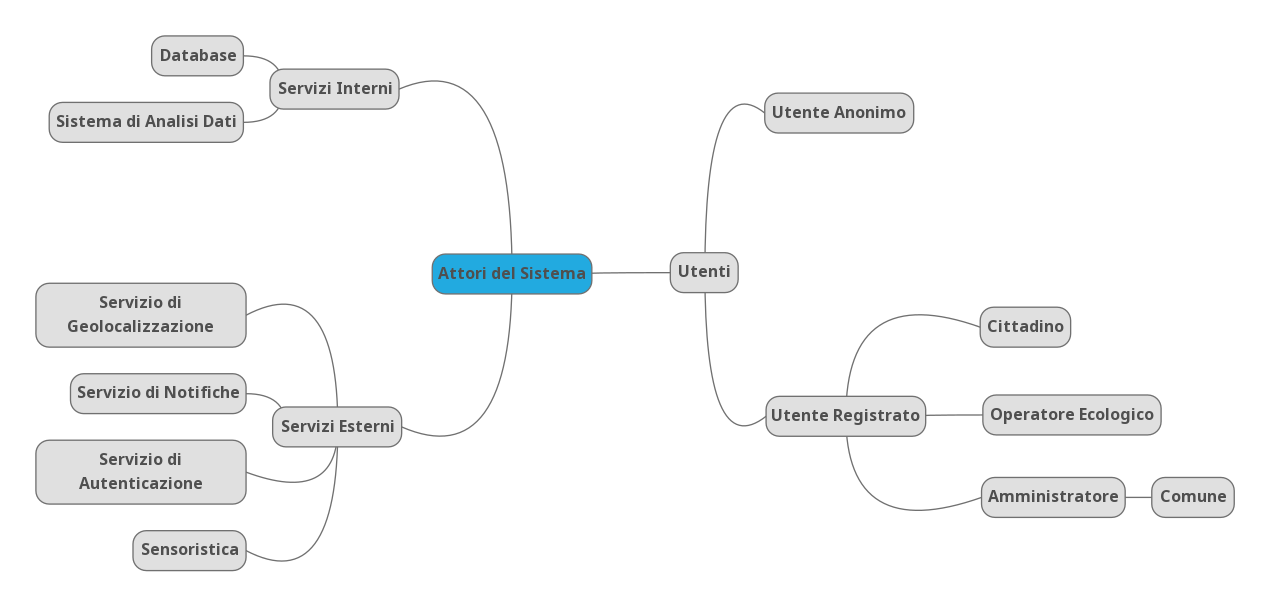
\includegraphics[width=1\linewidth]{D1-G1//Img/MindMap.png}
    \caption{Mind Map Attori del Sistema}
    \label{fig:enter-label}
\end{figure}

\subsection{Utenti}
    \subsubsection{Utente Anonimo}
    \begin{itemize}
        \item Utente con limitate funzionalità.
    \end{itemize}
    
    \subsubsection{Utente Registrato}
    \begin{itemize}
        \item \textbf{Cittadino}: \\ Può usufruire dei servizi dedicati alla popolazione.
        \item \textbf{Operatori Ecologico}: \\ Può usufruire dei servizi base e di alcuni servizi specifici.
        \item \textbf{Amministratore}: \\ Può visionare la dashboard che presenta dati statistici in merito alla gestione rifiuti della città.
    \end{itemize}

\subsection{Servizi Interni}
    \begin{itemize}
        \item \textbf{Database}: \\ Si occupa di salvare tutte le informazioni riguardanti gli utenti, la sensoristica, infrastrutture ecologiche e servizi al cittadino.
        \item \textbf{Analisi Dati}: \\ Il sistema utilizzato per elaborare i dati grezzi forniti dai sensori.
    \end{itemize}

\subsection{Servizi Esterni}
    \begin{itemize}
        \item \textbf{Servizio di Geolocalizzazione}: \\ Utilizzato per garantire all'utente non amministratore suggerimenti in base alla sua posizione.
        \item \textbf{Servizio di Notifiche}: \\ Utilizzato per raggiungere l'utente in merito ad eventi.
        \item \textbf{Servizio di Autenticazione}: \\ Utilizzato per registrare gli utenti e garantire una divisione basata sui permessi a loro assegnati.
        \item \textbf{Sensoristica}:\\ Utilizzato per fornire dati grezzi sulla situazione dei cassonetti, cestini ed ecocentri.
    \end{itemize}